\chapter{Results}
\label{cha:results}

This chapter will show some tests that have been done using two different cell sets. The first section is devoted to the use of the cells provided by the Nangate Open Cell Library, whereas the second section uses the \textit{CatLib Cell Library}. In both of them, tables regarding different CellDivider versions are presented and some conclusions are drawn. Given the number of possible experiments that could have been conducted, the ones presented have been selected to show the most important results of the work that has been done. A summary of the project's general conclusions will be presented in the next chapter. \\

Much testing was done during the development of the project. Each time a new version or variant was produced, it was tested with a set of representative cells of the Nangate library, about which we will explain more in Section \ref{sec:nangate}. Those experiments were generally done in the development laptop, given that the size of the Nangate instances is manageable using a normal computer. The experiments that will be shown in this chapter have been conducted on the LSI Cluster, using two Dell PowerEdge R410 using an Intel Xeon X5660 processor, with 12 cores and 2,8 Ghz frequency, and equipped with 96GB of RAM memory each. Using the cluster was advantageous over running the tests on the laptop for several reasons. Both nodes are equipped with high-end processors, so the computational time is lower. The main advantage is that, given the number of cores, many routing instances were solved in parallel. Besides, the memory of the system also mattered; there were routing instances that required more than 4GB of memory, which the laptop used for development could not provide. \\

\section{Nangate Open Cell Library}
\label{sec:nangate}

The first set is the Nangate Open Cell Library, which is the same that was used to test CellRouter. It is an open-source standard cell library provided for research purposes. It includes several  functions, for example buffers, combinational gates and flip-flops, all of which come in different drive strength variants. When referring to the name of a cell, first will come the name of the function followed by the drive strength (for example, an AND4\_X1 gate is a 4-input AND with the first level of drive strength). \\

A subset of the cells in the Nangate library has been selected for the purpose of making these experiments. The aim of this project is to help with big and complex cells. The cells that will be used are those that fall into one of such categories. The big ones cells are AND4\_X4, AOI22\_X4, BUF\_X32, INV\_X32, NOR4\_X4, OAI22\_X4 and OR4\_X4, whereas the complex cells, which are the most congested ones, are DFF\_X1, DFFR\_X1, DFFS\_X1, DFFRS\_X1, FA\_X1, SDFF\_X1, SDFFR\_X1, SDFFS\_X1 and SDFFRS\_X1. \\

Table \ref{tab:base_nangate} includes the routing time for all those cells using a halo of 6. We consider the case where the cell has not been optimized using heuristics and also when one or two optimization rounds have been done. The more heuristic optimization rounds are conducted, the higher the computational time becomes. The area is computed as the number of columns of the cell. \\


\begin{table}
\centering
\begin{tabular}{|l|r|r|r|r|}
\cline{1-5}
Cell & Area & No Optimization & 1 Round & 2 Rounds \\ \cline{1-5}
AND4\_X4 & 12 & 3,83 & 9,45 & 30,84  \\ \hline
AOI22\_X4 & 16 & 6,26 & 40,20 & 90,06  \\ \hline
BUF\_X32 & 24 & 33,03 & 155,20 & 290,97  \\ \hline
DFF\_X1 & 17 & 80,11 & 87,41 & 109,51  \\ \hline
DFFR\_X1 & 19 & 228,69 & 237,75 & 296,88  \\ \hline
DFFS\_X1 & 20 & 38,66 & 49,98 & 67,08  \\ \hline
DFFRS\_X1 & 24 & 150,58 & 175,56 & 221,56  \\ \hline
FA\_X1 & 15 & 30,11 & 35,28 & 45,11  \\ \hline
INV\_X32 & 32 & 13,37 & 58,56 & 107,15  \\ \hline
NOR4\_X4 & 16 & 5,64 & 23,21 & 54,40  \\ \hline
OAI22\_X4 & 16 & 6,36 & 13,64 & 49,27  \\ \hline
OR4\_X4 & 12 & 4,28 & 7,00 & 29,15  \\ \hline
SDFF\_X1 & 24 & 60,56 & 80,98 & 109,37  \\ \hline 
SDFFR\_X1 & 27 & 40,94 & 68,33 & 99,13  \\ \hline 
SDFFS\_X1 & 25 & 441,60 & 473,08 & 590,88  \\ \hline
SDFFRS\_X1 & 30 & 310,45 & 365,86 & 459,83  \\ \hline \cline{1-5}
\end{tabular} 
\caption{Time (s) used to solve Nangate cells}
\label{tab:base_nangate}
\end{table}


A first interesting experiment consists on simply dividing the cell in a half, routing the part on the right and then solving the whole cell together. Table \ref{tab:ncell_nangate} shows the obtained results. The numbers in the top row indicate the partial routing halo, the number of partial routing optimization rounds, final routing halo and the final routing optimization rounds. For example, the 6 0 12 0 column means that the right half of the cell has been routed with halo 6, has undergone 0 rounds of optimization, and that the final routing of the cell has been done using routing 12 also without any optimization round. The No Opt and 1 Round columns are the original times from Table \ref{tab:base_nangate}. A value of 0 indicates that the cell was found to be unroutable. \\

\begin{table}
\centering
\begin{tabular}{|l|r|r|r|r|r|r|}
\cline{1-7}
Cell & No Opt & 6 0 6 0 & 6 0 15 0 & 1 Round & 6 1 6 1 & 6 1 15 1 \\ \cline{1-7}
AND4\_X4 & 3,83 & 6,15 & 6,36 & 9,45 & 26,48 & 22,25  \\ \hline
AOI22\_X4 & 6,26 & 7,64 & 7,94 & 40,20 & 0 & 28,59  \\ \hline
BUF\_X32 & 33,03 & 25,62 & 25,62 & 155,20 & 119,2 & 176,8  \\ \hline
DFF\_X1 & 80,11 & 0 & 0 & 87,41 & 0 & 0  \\ \hline
DFFR\_X1 & 228,69 & 0 & 0 & 237,75 & 0 & 0  \\ \hline
DFFS\_X1 & 38,66 & 0 & 0 & 49,98 & 43,92 & 184,81  \\ \hline
DFFRS\_X1 & 150,58 & 0 & 0 & 175,56 & 0 & 0  \\ \hline
FA\_X1 & 30,11 & 12,68 & 27,33 & 35,28 & 0 & 0  \\ \hline
INV\_X32 & 13,37 & 12,32 & 17,77 & 58,56 & 42,7 & 60,58  \\ \hline
NOR4\_X4 & 5,64 & 6,36 & 9,08 & 23,21 & 22,94 & 28,34  \\ \hline
OAI22\_X4 & 6,36 & 0 & 9,63 & 13,64 & 0 & 30,21  \\ \hline
OR4\_X4 & 4,28 & 0 & 0 & 7,00 & 15,51 & 20,69  \\ \hline
SDFF\_X1 & 60,56 & 0 & 0 & 80,98 & 0 & 0  \\ \hline 
SDFFR\_X1 & 40,94 & 38,7 & 97,4 & 68,33 & 0 & 0  \\ \hline 
SDFFS\_X1 & 441,60 & 81,29 & 981,93 & 473,08 & 221,01 & 1242,59  \\ \hline
SDFFRS\_X1 & 310,45 & 0 & 0 & 365,86 & 0 & 0  \\ \hline \cline{1-7}
\end{tabular} 
\caption{Time (s) used to solve Nangate cells using the 2-Cell routing}
\label{tab:ncell_nangate}
\end{table}

It is important to notice the difference on behavior of the two kinds of cells, the big and the complex ones. Most of the cells are found to be routable in the first group, even though there are exceptions such as some cases in the AOI22\_X4, OAI22\_X4 and OR4\_X4 gates. However, in most of these cells there is no significant reduction in the amount of CPU time requiered to solve the cell, either in just routing it or obtaining a result with one round of optimization.  Notice how the versions with more allowed halo on the final routing find more valid solutions than the others. Similarly, when optimization is done to the partial routing, the total cell can switch from unroutable from routable, as in the case of OR4\_X4. \\

The case for the congested cells is different. Most of them happen to be unroutable using the 2-Cell approach. This is because the partial solution makes some decisions that do not allow a total routing to be found. However, when routed, some impressive time reductions are also achieved. In the case of FA\_X1, it is routed close to three times faster. An even more impressive result is the one for SDFFS\_X1, which took 441,6 seconds origianlly and can be routed with merely 81,29 seconds. Still most of the times the output happens to be unsatisfiable. Even when adding more halo to the final routing or optimizing to ease the process some routable results are lost, as happens with SDFFR\_X1 and FA\_X1. \\

It is unclear whether or not adding more optimization rounds leads to more satisfiable cells in the case of congested cells. When a partial solution is copied to the original cell, the parts in the boundary are the less congested ones. More optimization rounds are not meaningful to this areas. However, the sole fact that an optimized result may vary the position of the wires explains why some move from routable to unroutable as the number of cleaning rounds increases. \\

In general, we can see that using the 2-Cell routing schema leads to very good results in some cases but, in many others, fails to find a solution or does not reduce the computational time. \\

Table \ref{tab:window_nangate} shows the routing time in seconds using window congestion-driven routing. The No Opt column represents the original routing times without optimization. The numbers after ``Window'' represent the halo that was used for the partial routing and for the final total routing. \\

\begin{table}
\centering
\begin{tabular}{|l|r|r|r|}
\cline{1-4}
Cell & No Opt & Window, 6 6 & Window, 6 12 \\ \cline{1-4}
AND4\_X4 & 3,83 & 13,09 & 15,22 \\ \hline
AOI22\_X4 & 6,26 & 0 & 54,45 \\ \hline
BUF\_X32 & 33,03 & 0 & 0  \\ \hline
DFF\_X1 & 80,11 & 0 & 0  \\ \hline
DFFR\_X1 & 228,69 & 0 & 0  \\ \hline
DFFS\_X1 & 38,66 & 69,11 & 74,4  \\ \hline
DFFRS\_X1 & 150,58 & 173,93 & 1094,21  \\ \hline
FA\_X1 & 30,11 & 47,35 & 73,76 \\ \hline
INV\_X32 & 13,37 & 0 & 0 \\ \hline
NOR4\_X4 & 5,64 & 0 & 38,68  \\ \hline
OAI22\_X4 & 6,36 & 0 & 39,21  \\ \hline
OR4\_X4 & 4,28 & 0 & 0 \\ \hline
SDFF\_X1 & 60,56 & 0 & 48,68 \\ \hline 
SDFFR\_X1 & 40,94 & 0 & 0  \\ \hline 
SDFFS\_X1 & 441,60 & 0 & 0  \\ \hline
SDFFRS\_X1 & 310,45 & 0 & 0  \\ \hline \cline{1-4}
\end{tabular} 
\caption{Time (s) used to solve Nangate cells using window congestion-driven routing}
\label{tab:window_nangate}
\end{table}

The result is that most of the cells happen to be unsatisfiable. This can be partly solved by using a greater halo when routing the whole cell in the last step, but then the computation times rise too much. However, studying this case was interesting due to the potential in the use of congestion metrics to decide which parts to route. As explained before, the congestion-driven versions were left partway through development to center the effort in the scan algorithm, whose results follow now. \\

Table \ref{tab:scan_nangate} shows the results of using the scan meta-algorithm, partitioning in two parts. The first number above each column indicates the halo that was used when doing each routing and the second one indicates the number of optimization rounds each part underwent. The ``No Opt'' column represents the original routing time and the ``1 Round'' column represents the original time for routing and doing 1 round of optimization. \\

\begin{table}
\centering
\begin{tabular}{|l|r|r|r|r|r|r|}
\cline{1-7}
Cell & No Opt & 6 0 & 15 0 & 1 Round & 6 1 & 15 1 \\ \hline \cline{1-7}
AND4\_X4 & 3,83 & 0 & 0 & 9,45 & 15,49 & 21,01  \\ \hline
AOI22\_X4 & 6,26 & 11,59 & 8,58 & 40,20 & 24,18 & 19,47  \\ \hline
BUF\_X32 & 33,03 & 28,69 & 25,07 & 155,20 & 111,18 & 166,64  \\ \hline
DFF\_X1 & 80,11 & 0 & 0 & 87,41 & 0 & 51,34  \\ \hline
DFFR\_X1 & 228,69 & 0 & 0 & 237,75 & 0 & 0  \\ \hline
DFFS\_X1 & 38,66 & 0 & 0 & 49,98 & 0 & 0 \\ \hline
DFFRS\_X1 & 150,58 & 0 & 0 & 175,56 & 0 & 0  \\ \hline
FA\_X1 & 30,11 & 0 & 0 & 35,28 & 20,48 & 30,73  \\ \hline
INV\_X32 & 13,37 & 10,23 & 14,85 & 58,56 & 50,56 & 80,32  \\ \hline
NOR4\_X4 & 5,64 & 0 & 8,37 & 23,21 & 0 & 25,19  \\ \hline
OAI22\_X4 & 6,36 & 0 & 8,21 & 13,64 & 0 & 25,55  \\ \hline
OR4\_X4 & 4,28 & 0 & 7,06 & 7,00 & 0 & 0  \\ \hline
SDFF\_X1 & 60,56 & 23,21 & 0 & 80,98 & 0 & 0  \\ \hline 
SDFFR\_X1 & 40,94 & 0 & 0 & 68,33 & 30,86 & 0  \\ \hline 
SDFFS\_X1 & 441,60 & 0 & 0 & 473,08 & 0 & 0  \\ \hline
SDFFRS\_X1 & 310,45 & 0 & 0 & 365,86 & 0 & 0  \\ \hline \cline{1-7}
\end{tabular} 
\caption{Time (s) used to solve Nangate cells using scan routing}
\label{tab:scan_nangate}
\end{table}

As happenes with the case presented before, a large number of cells turns out to be unsatisfiable for the last routing step. We can observe that most of the big cells are routable but no gain in performance is obtained except in the case of AOI22\_X4 and BUF\_X32, where time has dropped to a half in the first case and to two thirds in the second case. \\

It is interesting to focus again on the more complex cells. Once again, in most of the configurations we happen to find unsatisfiable final problems. However, when a satisfiable solution is found, it is faster than when using normal routing on the cells. This is the case of DFF\_X1, FA\_X1, SDFF\_X1 and SDFFR\_X1. Each of these cells has been routed using from three quarters to a mere third of the original routing time. In some of the cases, not only has the computational time been reduced compared to the version where optimization is done, but even when compared to simply routing the cell. \\


Experimentation with this subset of cells, which is representative of the Nangate cells that we want to tackle in this project, has provided interesting results. On one hand we have learned how thin the barrier between a solution leading to unsatisfiable global routings and one leading to an overall valid solutions is. On the other hand, we see that the divide-and-conquer approach has achieved much time reduction in the case of big Nangate cells, whereas it shows to be powerful on the most congested cells when it manages to find a valid solution. Next section explores what happens with cells which are bigger than the ones offered by the Nangate library. \\

\section{CatLib Cell Library}

The second set of cells consists of the concatenation of Nangate cells which have been grouped under the name of \textit{CatLib}. They have been created on purpose to test several properties of the divide-and-conquer algorithms given that we wanted to test the tool on cells bigger than those offered by the Nangate library. \\

In order to do so, \textit{CellCat}, a basic cell concatenation tool, has been developed. It outputs the concatenation of a given number of instances of the cell. When choosing which cells should be on CatLib we wanted to focus on two kind of cells again, depending on whether they were heavily congested or not. An analysis of the whole Nangate library was conducted to determine which cells would be useful to generate bigger cells with the lowest congestion possible. To select these cells, both the mean number of subnets that crossed each column and the total size of the cell were considered. Finally, NOR4\_X4 and OAI22\_X4 where chosen. In the case of the congested cells, given that the time of solving each cell by the original tool was known, those which proved to be hard were selected: The FA\_X1 full adder cell and various flip-flops. When referring to a CatLib cell, the nomenclature NAME\_N will indicate the cell that was concatenated in NAME and the times it was included in N. For exmaple, the FA\_X1\_3 cell is the concatenation of three full adder cells. \\

Finally, CatLib cells can be divided into three groups: Combinational cells, full adders and flip-flops. The first case simply considers the concatenation of some combinational cells (\textit{COMB} in Figure \ref{fig:NCombinacionals}) which share up to one signal. These should prove to be the easiest to route given that close to no congestion should exist in the region between cells. \\

\begin{figure}[h!]
  \centering
  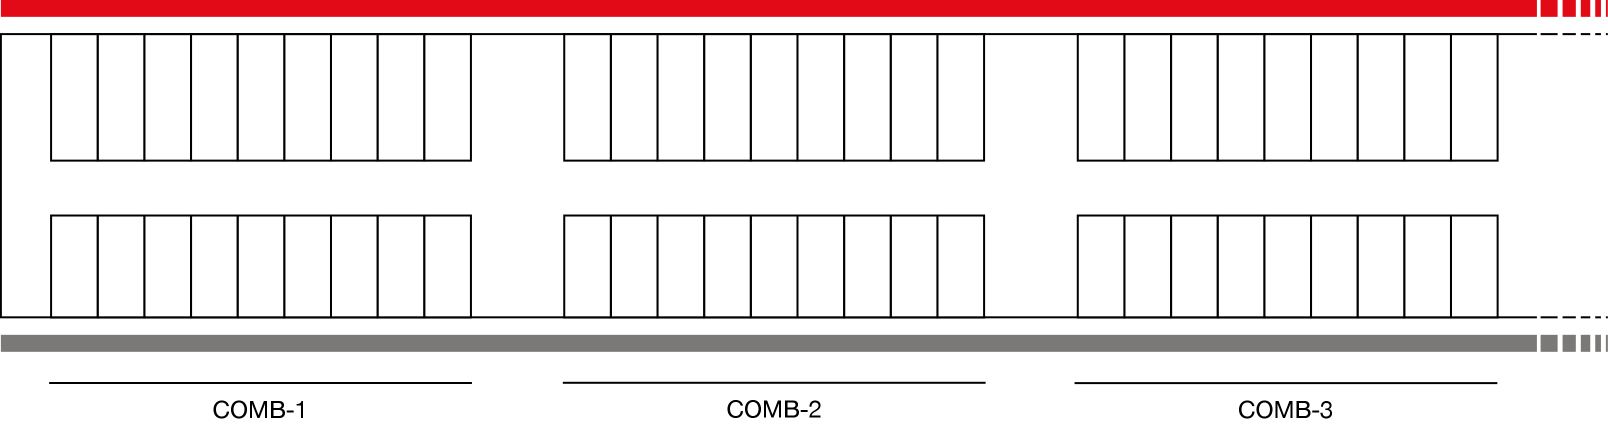
\includegraphics[scale=0.5]{img/results/NCombinacionals.png}
  \caption{Concatenation of combinational cells}
  \label{fig:NCombinacionals}
\end{figure} 

In the second case, where 1-bit full adders are concatenated, the carry out signal of a given full adder has to be connected with the carry in of the next full adder, with the exception of the first carry in and the last carry out which are terminals of the final cell. In Figure \ref{fig:FA_X1_N} it can be seen how a routing of a $n$-bit full adder might look like. \\

\begin{figure}[h!]
  \centering
  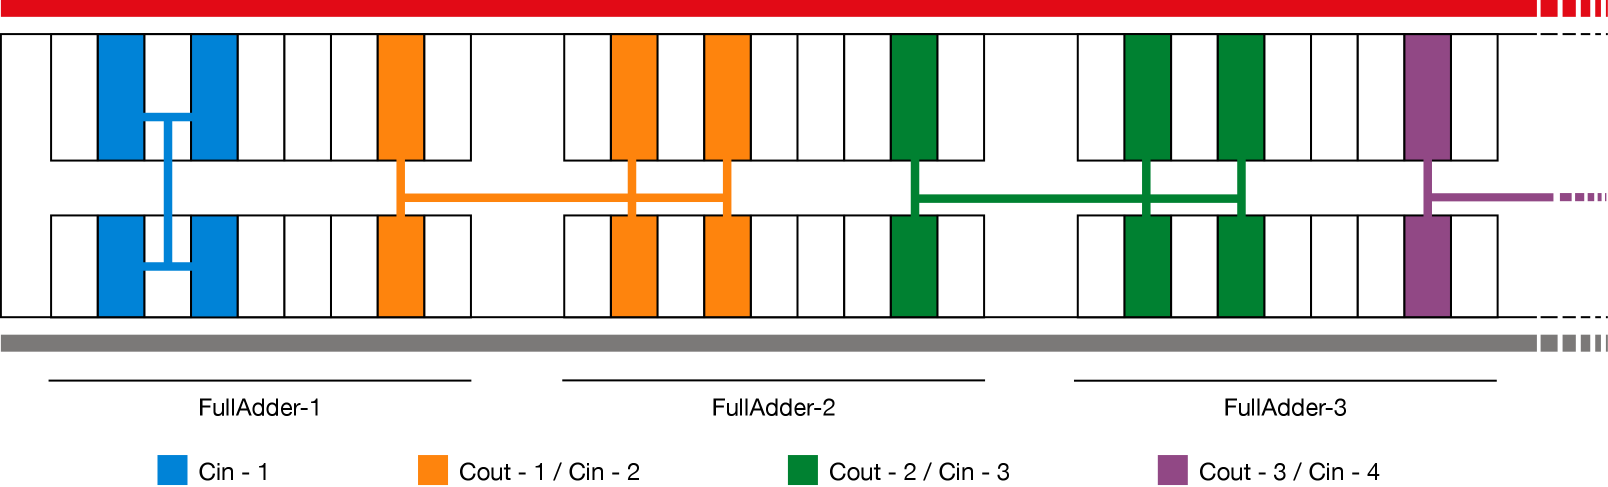
\includegraphics[scale=0.5]{img/results/FA_X1_N.png}
  \caption{Concatenation of full adders cells}
  \label{fig:FA_X1_N}
\end{figure} 

The last case is the concatenation of 1-bit flip-flops, generating a $n$-bit flip-flop cell. This time we do not need to carry signals from one region to the next one, but we need to share signals across the whole cell. The most basic flip-flop only needs to share the clock signal, but up to five signals need to cross the whole cell in the case of scan flip-flop with set and reset, as is the case of the SDFFRS cells. In Figure \ref{fig:Flipflop_N}, the concatenation with a possible routing of reset flip-flops is shown. \\
  	
\begin{figure}[h!]
  \centering
  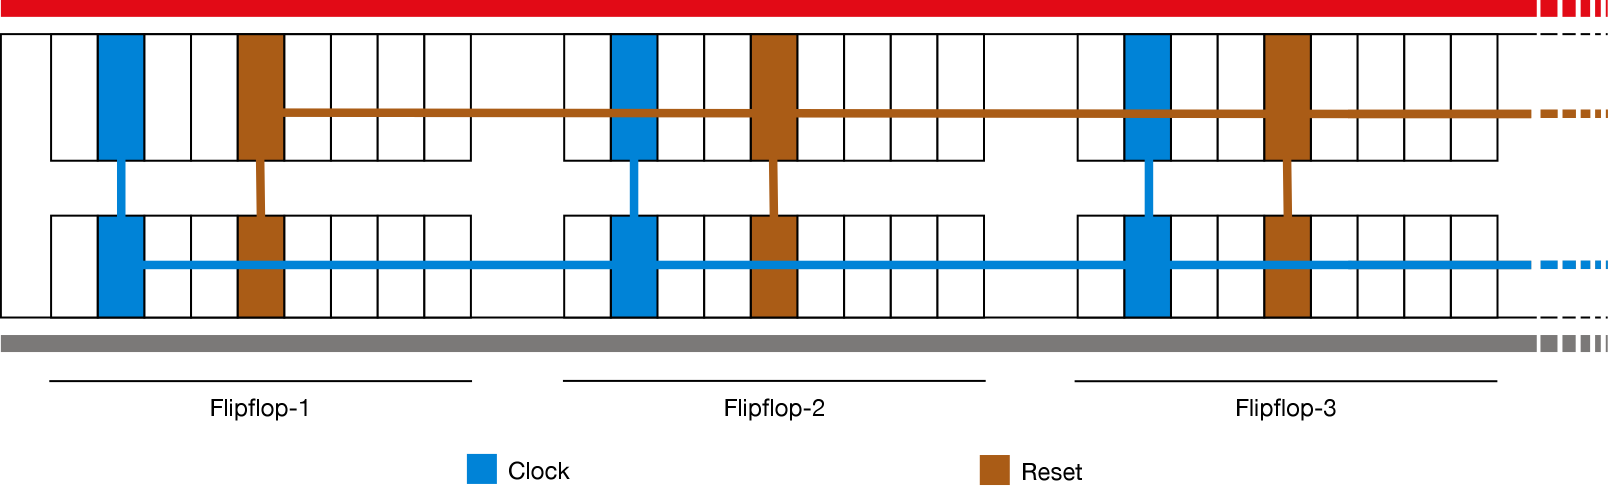
\includegraphics[scale=0.5]{img/results/Flipflop_N.png}
  \caption{Concatenation of reset flip-flops}
  \label{fig:Flipflop_N}
\end{figure} 
  	

These cells were routed in the cluster using various halo sizes. Table \ref{tab:base_concat} shows the routing time in seconds for the adders and flip-flops using a halo of 2. The numbers on the columns indicate how many times each cell was concatenated. Originally no more than the concatenation of 4 cells was used, given the enormous time it took to solve smaller cases, except for the case of NOR4\_X4 and OAI22\_X4, where up to 8 cells were concatenated. Table \ref{tab:base_combintional} shows the routing time in seconds and the maximum consumed memory in GBytes for these two cells. \\


\begin{table}
\centering
\begin{tabular}{|l|r|r|r|r|}
\cline{1-5}
Cell & 1 & 2 & 3 & 4 \\ \cline{1-5}
FA\_X1 & 17,05 & 101,95 & 316,96 & 1440,18 \\ \hline
DFF\_X2 & 10,4 & 74,14 & 221,16 & 726,14 \\ \hline
DFFS\_X1 & 22,25 & 289,59 & 2644,04 & 14138,55 \\ \hline
DFFS\_X2 & 14,38 & 398,74 & 2018,35 & 8542,4 \\ \hline \cline{1-5}
\end{tabular} 
\caption{Time (s) used to solve concatenated adders and flip-flop}
\label{tab:base_concat}
\end{table}


\begin{table}
\centering
\begin{tabular}{|l|r|r|r|r|r|r|r|r|}
\cline{1-9}
Cell & 1 & 2 & 3 & 4 & 5 & 6 & 7 & 8\\ \cline{1-9}
\multirow{2}{*}{NOR4\_X4} & 4,8 & 21,6 & 71,53 & 127,23 & 295,46 & 482,79 & 695,27 & 962,64\\
& 0,19 & 0,48 & 1,1 & 1,94 & 3,47 & 5,35 & 7,66 & 10,62  \\ \hline
\multirow{2}{*}{OAI22\_X4} & 6,8 & 35,78 & 92,41 & 213,17 & 381,42 & 597,23 & 984,24 & 1407,86 \\
& 0,19 & 0,57 & 1,72 & 3,63 & 6,38 & 7,97 & 14,16 & 21,35 \\ \hline \cline{1-9}
\end{tabular} 
\caption{Time (s) and memory (GB) used to solve concatenated cells}
\label{tab:base_combintional}
\end{table}

Additionally, another kind of cell is considered. It consists not on the concatenation, but the fusion of several cells having some signals in common. These gates can share their inputs, outputs or both. Figure \ref{fig:hax_schematic} represents the schematic view of how such a cell could be. This cell, named \textit{HAX}, has been used to test how CellDivider would act in front of the combination of arbitrary different combinational cells. It has 134 columns and 51 different signals. Its purpose is solely to illustrate what happens with a cell that has no regular structure, such as concatenated cells, and which has several components that share signals or must be crossed by other signals.

\begin{figure}[h!]
  \centering
  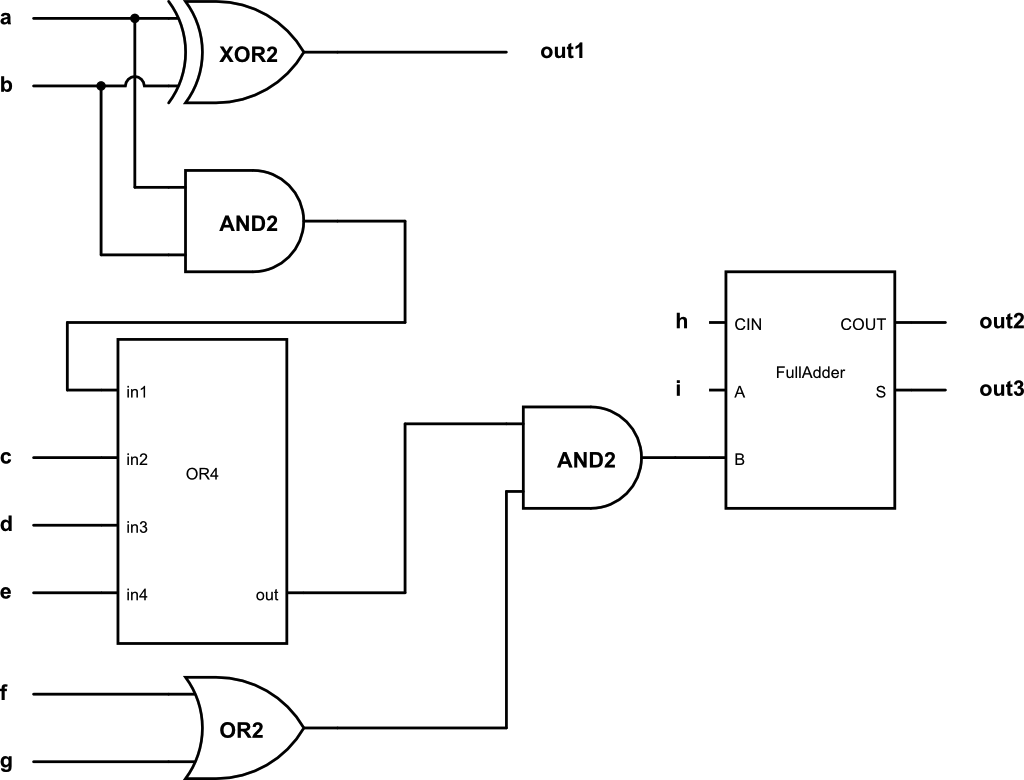
\includegraphics[scale=0.3]{img/results/hax_schematic.png}
  \caption{HAX gate - Schematic view}
  \label{fig:hax_schematic}
\end{figure} 


\subsection{Combinational Cells}

When dealing with the combinational cells, the scan routing algorithm proved to work very well. Each cell was divided into the number of original gates it contained and they were routed one after another. Given that no signal is shared among them, these routings can be done very easily and with close to no extra congestion. Table \ref{tab:goodcombinatiornal} shows the time values that were obtained. The number on each column represents how many cells were concatenated in each case. \\

\begin{table}
\centering
\begin{tabular}{|l|r|r|r|r|r|r|r|r|}
\cline{1-9}
Cell & 1 & 2 & 3 & 4 & 5 & 6 & 7 & 8\\ \cline{1-9}
NOR4\_X4 & 8,27 & 16,36 & 24,43 & 33,51 & 41,9 & 50,7 & 59,42 & 68,77\\ \hline
OAI22\_X4 & 9,56 & 18,94 & 28,45 & 37,86 & 47,41 & 58,19 & 68,87 & 77,68 \\\cline{1-9}
\end{tabular} 
\caption{Concatenated combinational cells - Time (s) used}
\label{tab:goodcombinatiornal}
\end{table}

As it can be easily seen, they follow a linear relation with the number of cells that get routed. Another interesting result comes in terms of used memory. When routing all the gates no more than 300Mbytes were used, which is negligible compared to how much memory (up to 21 GB) was used by the biggest cells when routing them directly.  \\

These are good results, but are applied to a very restricted and simple case. Consider now the combinational cells where each cell shares a signal with the following one. This case is a little more complex because, now, the parts are not so independent from each other. NORN\_X4 is a gate composed of the concatenation of NOR4\_X4 gates sharing a signal, as described before. Table \ref{tab:norn} includes the time in seconds for finding a valid solution and additionally performing an optimization round with CellRouter. It also contains the time used for the scan algorithm to find a valid routing for the cell using halo 6. It must be kept in mind that scan algorithm outputs already optimized cells given that it performs optimization in every partial routing. It can be seen how, despite performing worse in the case of the smaller cells, scan routing does a better job when they become bigger. When dividing the cell with 8 NORN gates we obtain an unsat result with halo 6 as shown in the table, but by using a halo of 10 it can be routed in 500 seconds. \\

\begin{table}
\centering
\scalebox{0.85}{%
\begin{tabular}{|l|r|r|r|r|r|r|r|r|}
\cline{1-9}
Method & 1 & 2 & 3 & 4 & 5 & 6 & 7 & 8 \\ \cline{1-9}
Route & 4,74 & 20,81 & 65,33 & 122,89 & 230,73 & 427,72 & 636,21 & 931,03\\ \hline
Route and optimize & 20,84 & 144,92 & 184,59 & 410,05 & 713,03 & 1320,29 & 2056,7 & 2704,96\\ \hline
Scan Algorithm & 24,8 & 52,39 & 112,65 & 149,16 & 231,24 & 265,28 & 278,91 & unsat \\\cline{1-9}
\end{tabular}}
\caption{Concatenated NORN\_X4 gates - Time (s) used}
\label{tab:norn}
\end{table}

Figure \ref{fig:norn} shows a graphic displaying the values of the table. The number on the column represents the number of concatenated NORN\_X4 cells. It can be seen how, despite performing worse in the case of the smaller cells, scan routing does a better job when they become bigger. \\

\begin{figure}[h!]
  \centering
  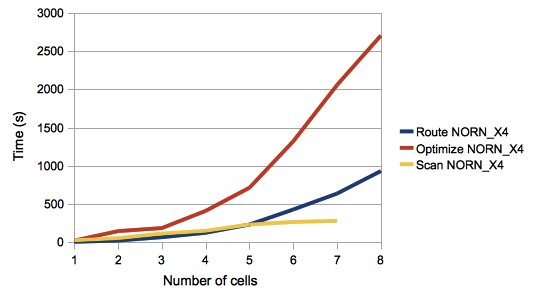
\includegraphics[scale=0.7]{img/results/norn.png}
  \caption{NORN\_X4 gate - Solving time comparison}
  \label{fig:norn}
\end{figure} 

\subsection{Full adders}

The case for concatenated full adders is more complicated. Not only is a signal shared with each full adder on both sides, but also the full adder standard cell is a very congested one. When experimenting with the scan algorithm, in many of the cases the result was unsat. This is because some partial routings did a bad choice and the algorithm was not able to find a valid solution. \\

However, some positive results were achieved. With a halo of 15 and partitioning the cell in the same number of concatenated full adders that it contained, the results are as shown in Table \ref{tab:scanadder}. The number on the column represents the number of concatenated FA\_X1 cells. Each partial solution used two optimization rounds so that the probability of a finding a valid assignment raised. \\


\begin{table}
\centering
\begin{tabular}{|l|r|r|r|r|r|r|r|r|}
\cline{1-7}
Method & 1 & 2 & 3 & 4 & 5 & 6\\ \cline{1-7}
Route & 17,05 & 101,95 & 316,96 & 1440,18 & 2127,56 & 4985,79 \\ \hline
Route and optimize & 24,62 & 150,27 & 545,79 & 1636,00 & 2430,75 & 6697,23 \\ \hline
Scan Algorithm & 39,42 & 92,33 & 163,84 & 257,54 & 395,02 & unsat\\ \cline{1-7}
\end{tabular}
\caption{Concatenated FA\_X1 gates - Time (s) used}
\label{tab:scanadder}
\end{table}

The trend of all the methods can be seen in Figure \ref{fig:scanadder}. Note that the execution time of the scan routing version outperforms the direct routing from 2 concatenated full adders. When routing with different halos, most of the times the result happened to be non routable. The number of unsatisfiable final results is very high and several combinations of halo and number of divisions have to be explored to finally route the full adder cells. \\

\begin{figure}[h!]
  \centering
  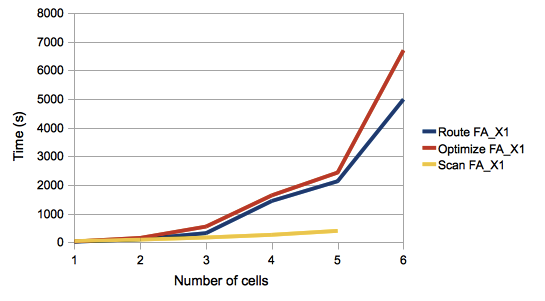
\includegraphics[scale=0.7]{img/results/scanadder.png}
  \caption{FA\_X1\_N gate - Solving time comparison}
  \label{fig:scanadder}
\end{figure} 

\subsection{Filp-flops}

The flip-flop cells are the most difficult to route. Results with flip-flop concatenations have reflected this clearly. These cells share from 1 signal, in the case of the DFF cells, to 5 signals, in the case of the SDFFRS cells. The more signals each concatenated cell has to share with the others, the more complex is for the complete cell to be routed. No cell where its components shared more than 2 elements was routable. In fact, considering only the concatenation of two flip-flop cells, the only ones that were routed are DFF\_X2, DFFS\_X1, DFFS\_X2 and DFFR\_X2. Even when trying to route them using different halos and algorithms, hardly any of them gave satisfiable solutions.  In the case of DFF\_X2, it was routed with the scan algorithm using halo 50, up to DFF\_X2\_4. The results can be seen on Table \ref{tab:scandff}. The number on the column represents the number of concatenated DFF\_X2 cells.\\

\begin{table}
\centering
\begin{tabular}{|l|r|r|r|r|r|r|}
\cline{1-5}
Method & 1 & 2 & 3 & 4\\ \cline{1-5}
Route & 10,4 & 74,14 & 221,16 & 724,14\\ \hline
Route and optimize & 16,11 & 130,47 & 483,13 & 1324,17\\ \hline
Scan Algorithm & 28,68 & 131,36 & 301,13 & 476,69\\ \cline{1-5}
\end{tabular}
\caption{Concatenated DFF\_X2 gates - Time (s) used}
\label{tab:scandff}
\end{table}

As happened with the case of the full adders, a lot of unsatisfiable results appear, specially when the number of divisions done to the cell is big. Aside from the particular case of DFF\_X2 and the concatenation of two DFFS cells, no satisfying results for the concatenated flip-flops were found. \\

\subsection{HAX Gate}

This cell is used as an example of an unstructured big and not very congested cell. Each original part of the cell shares from none to two signals with the parts next to it. Using a halo of 2 it can be routed in 208,29 seconds, having a total wirelength of 1784 wire segments. Applying one round of optimization, the computational time ascends to 511,81 seconds but the wirelength is reduced to 874, less than a half. Table \ref{tab:hax_table} shows the results of routing it using the scan algorithm with halos 2 and 6, partitioning the cell in 2, 3 or 4 parts. \\

\begin{table}
\centering
\begin{tabular}{|l|r|r|r|r|}
\cline{1-4}
 & 2 parts & 3 parts & 4 parts \\ \cline{1-4}
Halo 2 & 301,6 & unsat & 107,72 \\ \hline
Halo 6 & 341,98 & 254,96 & 135,37 \\ \cline{1-4}
\end{tabular}
\caption{HAX gate - Time (s) used}
\label{tab:hax_table}
\end{table}

When partitioning the cell in 4 parts it is routed in half the time that was used before. However, the wirelength is of 904 wire segments, which is comparable to the normal routing using one round of optimization, and has been obtained 5 times faster.


We can observe that when partitioning the cell into 3 parts using a low halo we obtain an unsatisfiable solution. The same happens when routing it with more than 5 parts. This is because of the same reason that caused unsatisfiability when dealing with the concatenated cells: congestion on the zone of the cut. The division in 4 parts cuts the cell in pieces which are not as highly congested as the ones on the other division possibilities. \\


\section{Conclusions}

As a conclusion, we can say that the divide-and-conquer scheme works well for many cells but, the more congested they become, the harder it is to find a valid global routing. However, when it is found, it is up to many times faster than it was using other methods such as directly using the complete boolean formula. In the next chapter, conclusions on the whole project will be given and possible future work lines will be discussed. \\